% =============================================================================
%  The Mathematics of demo.py -- a 7-microphone streaming beamformer
%  Build:  pdflatex beamformer_math.tex   (run twice for references / TOC)
%  Code excerpts are pulled live from demo.py, which must sit in this folder.
% =============================================================================
\documentclass[11pt]{article}

\usepackage[margin=1in]{geometry}
\usepackage[T1]{fontenc}
\usepackage{lmodern}
\usepackage{microtype}
\usepackage{amsmath,amssymb,amsthm,mathtools,bm}
\usepackage{booktabs,array}
\usepackage{xcolor}
\usepackage{listings}
\usepackage{caption,subcaption}
\usepackage{tikz}
\usetikzlibrary{arrows.meta,calc,positioning,decorations.pathreplacing,angles,quotes}
\usepackage{pgfplots}
\pgfplotsset{compat=1.18}
\usepgfplotslibrary{polar}
\usepackage[most]{tcolorbox}
\usepackage[colorlinks=true,linkcolor=blue!50!black,urlcolor=blue!50!black,citecolor=blue!50!black]{hyperref}

% ---------- theorem-like environments ----------------------------------------
\theoremstyle{plain}
\newtheorem{proposition}{Proposition}[section]
\theoremstyle{definition}
\newtheorem{definition}[proposition]{Definition}
\theoremstyle{remark}
\newtheorem{remark}[proposition]{Remark}

% ---------- design-rationale box ---------------------------------------------
\newtcolorbox{rationale}[1][]{breakable, enhanced, colback=orange!4, colframe=orange!60!black,
  boxrule=0.6pt, arc=2pt, left=6pt, right=6pt, top=4pt, bottom=4pt,
  title={Design rationale#1}, fonttitle=\bfseries\small, coltitle=black, colbacktitle=orange!15}
\newtcolorbox{intuition}{breakable, enhanced, colback=blue!3, colframe=blue!50!black,
  boxrule=0.6pt, arc=2pt, left=6pt, right=6pt, top=4pt, bottom=4pt,
  title={Intuition}, fonttitle=\bfseries\small, coltitle=black, colbacktitle=blue!10}

% ---------- notation ---------------------------------------------------------
\newcommand{\herm}{^{\mathsf H}}
\newcommand{\tr}{^{\mathsf T}}
\newcommand{\vw}{\mathbf{w}}
\newcommand{\vd}{\mathbf{d}}
\newcommand{\vx}{\mathbf{X}}
\newcommand{\vn}{\mathbf{V}}
\newcommand{\vp}{\mathbf{p}}
\newcommand{\vu}{\mathbf{u}}
\newcommand{\one}{\mathbf{1}}
\newcommand{\mI}{\mathbf{I}}
\newcommand{\G}{\bm{\Gamma}}
\newcommand{\Gmu}{\bm{\Gamma}_{\!\mu}}
\newcommand{\E}{\mathbb{E}}
\newcommand{\code}[1]{\texttt{\detokenize{#1}}}
\newcommand{\WNG}{\mathrm{WNG}}
\newcommand{\DI}{\mathrm{DI}}

% ---------- code listings ----------------------------------------------------
\lstset{language=Python, basicstyle=\ttfamily\footnotesize, numbers=left,
  numberstyle=\tiny\color{gray}, numbersep=6pt, keywordstyle=\color{blue!70!black},
  commentstyle=\color{green!40!black}, stringstyle=\color{red!60!black},
  frame=single, rulecolor=\color{gray!50}, framexleftmargin=2pt, xleftmargin=12pt,
  breaklines=true, columns=fullflexible, keepspaces=true, showstringspaces=false}
\newcommand{\demolines}[2]{\lstinputlisting[firstline=#1,lastline=#2,firstnumber=#1]{demo.py}}

% ---------- figure styles ----------------------------------------------------
\tikzset{arr/.style={-{Stealth[length=2.2mm]}, thick}}
\definecolor{sdcol}{RGB}{200,70,30}
\definecolor{dascol}{RGB}{40,90,170}

\title{\textbf{The Mathematics of \texttt{demo.py}}\\[4pt]
\large A 7-microphone superdirective beamformer, streamed through an overlap-add STFT}
\date{\today}

\begin{document}
\maketitle

\begin{abstract}
\noindent
\texttt{demo.py} turns the seven MEMS microphones of a miniDSP UMA-8 into one ``acoustic zoom lens''
pointed at the front of the board, and plays the result to headphones in real time.
This document derives every equation the program uses, from the plane-wave model through the
superdirective weight design to the short-time Fourier transform (STFT) that streams it.
Each section works the same way: \emph{intuition} first, then a \emph{derivation}, then a
\emph{code map} with the exact lines of \texttt{demo.py}, then the \emph{design rationale}
behind the parameter choices. All plotted numbers were computed from the code itself
(\texttt{design\_weights}, \texttt{steering\_vectors}), so the figures match what
\texttt{python demo.py --pattern} prints.
\end{abstract}

\tableofcontents

% =============================================================================
\section{Overview}\label{sec:overview}
% =============================================================================

Sound from a talker in front of the array reaches the seven microphones at slightly
different times. The pattern of delays depends only on the direction the sound comes from.
In the frequency domain each delay becomes a phase rotation. So at every frequency,
``listening in a direction'' means choosing seven complex weights that make the phasors
from the look direction add up exactly, while phasors from other directions partly cancel.
Figure~\ref{fig:pipeline} shows the complete signal chain.

\begin{figure}[ht]
\centering
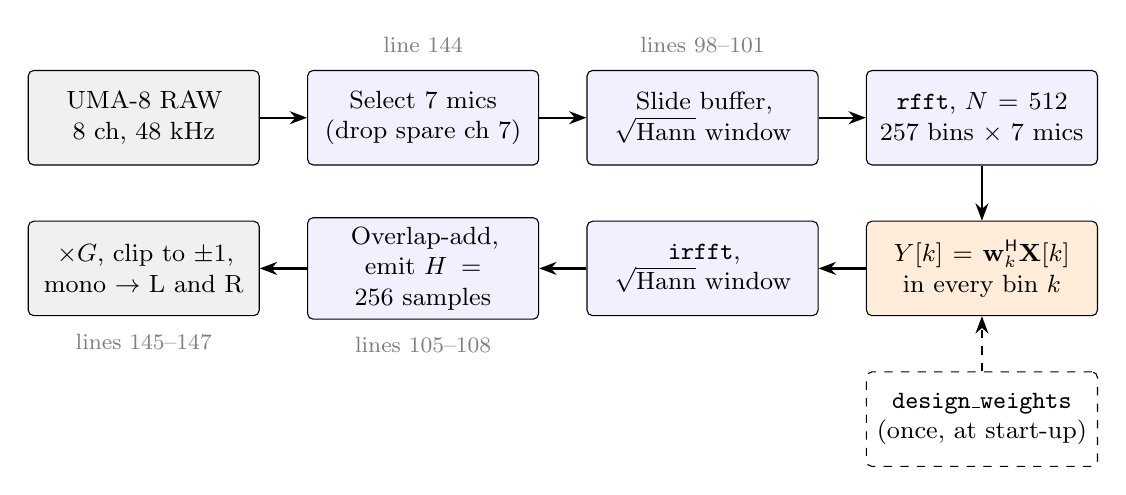
\begin{tikzpicture}[
  blk/.style={draw, rounded corners=2pt, fill=blue!6, align=center, font=\small,
              minimum height=12mm, text width=27mm},
  node distance=7mm and 6mm]
  \node[blk, fill=gray!12] (mic) {UMA-8 RAW\\8 ch, 48 kHz};
  \node[blk, right=of mic] (sel) {Select 7 mics\\(drop spare ch 7)};
  \node[blk, right=of sel] (ana) {Slide buffer,\\$\sqrt{\text{Hann}}$ window};
  \node[blk, right=of ana] (fft) {\texttt{rfft}, $N=512$\\$257$ bins $\times$ 7 mics};
  \node[blk, below=of fft, fill=orange!15] (bf) {$Y[k]=\vw_k\herm \vx[k]$\\in every bin $k$};
  \node[blk, left=of bf] (ifft) {\texttt{irfft},\\$\sqrt{\text{Hann}}$ window};
  \node[blk, left=of ifft] (ola) {Overlap-add,\\emit $H=256$ samples};
  \node[blk, left=of ola, fill=gray!12] (out) {$\times G$, clip to $\pm1$,\\mono $\to$ L and R};
  \node[blk, below=of bf, dashed, fill=white] (wd) {\texttt{design\_weights}\\(once, at start-up)};
  \draw[arr] (mic) -- (sel);  \draw[arr] (sel) -- (ana);  \draw[arr] (ana) -- (fft);
  \draw[arr] (fft) -- (bf);   \draw[arr] (bf) -- (ifft);  \draw[arr] (ifft) -- (ola);
  \draw[arr] (ola) -- (out);  \draw[arr, dashed] (wd) -- (bf);
  \node[font=\footnotesize, gray, below=1mm of out] {lines 145--147};
  \node[font=\footnotesize, gray, below=1mm of ola] {lines 105--108};
  \node[font=\footnotesize, gray, above=1mm of ana] {lines 98--101};
  \node[font=\footnotesize, gray, above=1mm of sel] {line 144};
\end{tikzpicture}
\caption{The signal chain in \texttt{demo.py}. Every audio callback receives $H=256$ new samples
per channel and returns $H$ output samples. The weights are computed once.}
\label{fig:pipeline}
\end{figure}

\paragraph{Notation.}
$M=7$ microphones; sample rate $f_s=48\,000$\,Hz; hop $H=256$; FFT length $N=2H=512$;
speed of sound $c=343$\,m/s; ring radius $r=0.043$\,m. Bold lower-case letters are column
vectors in $\mathbb{C}^M$ (one entry per microphone). $(\cdot)\tr$ is the transpose and
$(\cdot)\herm$ the conjugate transpose. Frequency bin $k\in\{0,\dots,N/2\}$ has centre
frequency $f_k=k f_s/N=k\cdot 93.75$\,Hz. The acoustic wavenumber is $\kappa=2\pi f/c$
(rad/m); the letter $k$ is reserved for the bin index. Table~\ref{tab:codemap} maps each part
of the code to a section of this document.

\begin{table}[ht]
\centering\small
\begin{tabular}{@{}llll@{}}
\toprule
Code object & Lines & What it computes & Section\\
\midrule
constants & 6--35 & geometry, physics, gains & \ref{sec:geometry}, App.~\ref{app:params}\\
\code{mic_layout} & 48--55 & mic positions $\vp_m$ & \ref{sec:geometry}\\
\code{steering_vectors} & 58--63 & $\vd(f,\phi)$ & \ref{sec:steering}\\
\code{design_weights} (\code{das}) & 72--73 & $\vw=\vd/M$ & \ref{sec:das}\\
\code{design_weights} (superdirective) & 75--82 & $\vw=\Gmu^{-1}\vd/(\vd\herm\Gmu^{-1}\vd)$ & \ref{sec:sd}\\
\code{print_beampattern} & 112--131 & $B(f,\phi)$, WNG & \ref{sec:pattern}\\
\code{StreamingBeamformer} & 85--109 & STFT, overlap-add & \ref{sec:stft}\\
\code{audio_callback}, \code{main} & 135--147, 196--201 & gain, clip, routing & \ref{sec:gain}\\
\code{show_levels} & 150--167 & per-channel dBFS & \ref{sec:gain}\\
\bottomrule
\end{tabular}
\caption{Where each piece of \texttt{demo.py} is explained.}
\label{tab:codemap}
\end{table}

\begin{rationale}[: why work in the frequency domain?]
The delays involved are tiny. The largest is $r/c\approx125\,\mu$s, about 6 samples, and most
are a fraction of a sample. A fractional delay is awkward in the time domain (it needs an
interpolation filter) but exact in the frequency domain: it is just a phase factor.
The superdirective weights are also \emph{frequency-dependent by design}
(Section~\ref{sec:sd}), so a per-bin design is the natural form. The STFT gives both, at the
cost of one $N$-point FFT per channel per hop.
\end{rationale}

% =============================================================================
\section{Array geometry}\label{sec:geometry}
% =============================================================================

\demolines{12}{29}

The UMA-8 has one centre microphone and six on a hexagon of radius $r=43$\,mm
(Figure~\ref{fig:array}). The axes are $x$ = front (away from the USB cable) and $y$ = left,
and azimuth $\phi$ is measured from the front, positive to the left. Mic $m$ on the ring at
angle $\theta_m$ sits at
\begin{equation}\label{eq:positions}
  \vp_m = r\begin{bmatrix}\cos\theta_m\\ \sin\theta_m\end{bmatrix},\qquad
  \vp_0=\begin{bmatrix}0\\0\end{bmatrix}.
\end{equation}

\demolines{48}{55}

Line~52 evaluates \eqref{eq:positions} for all six ring mics at once.
\code{np.stack(..., axis=1)} builds a $6\times2$ matrix with one row per mic.
Line~53 prepends the centre mic, so \code{positions} is $7\times 2$, and row $m$ belongs to
USB channel \code{channels[m]}.

\begin{figure}[ht]
\centering
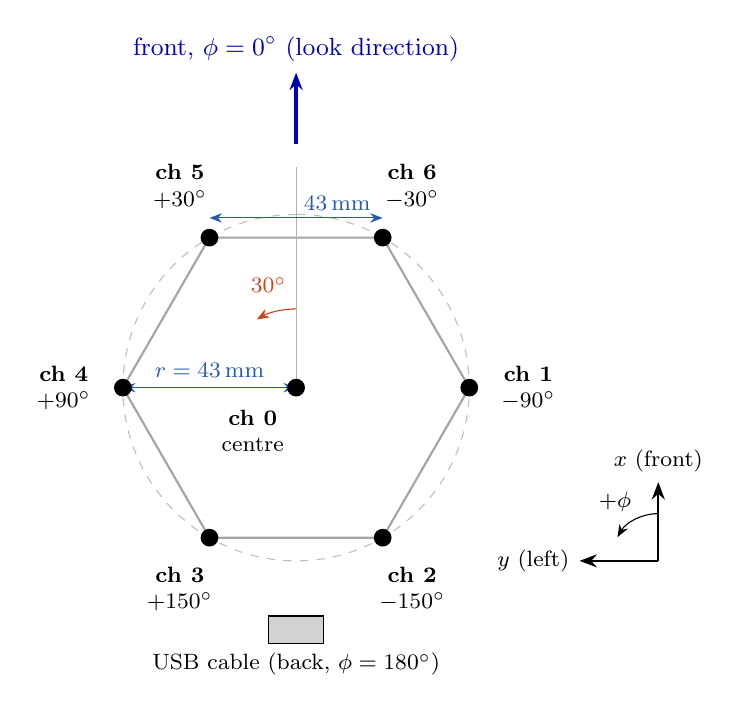
\begin{tikzpicture}[scale=1.0]
  \def\R{2.2}
  % front arrow and USB connector (unrotated: front is up)
  \draw[arr, blue!70!black, line width=1.2pt] (0,\R+0.9) -- (0,\R+1.8)
       node[above, font=\small] {front, $\phi=0^\circ$ (look direction)};
  \draw[fill=gray!35] (-0.35,-\R-1.05) rectangle (0.35,-\R-0.7);
  \node[font=\footnotesize, below] at (0,-\R-1.05) {USB cable (back, $\phi=180^\circ$)};
  \begin{scope}[rotate=90]   % inside: (theta:rad) puts theta=0 at screen-up, + to the left
    \draw[gray!50, dashed] (0,0) circle (\R);
    \draw[gray!70, thick] (90:\R) -- (30:\R) -- (-30:\R) -- (-90:\R) -- (-150:\R) -- (150:\R) -- cycle;
    \draw[gray!60] (0,0) -- (0:\R+0.6);
    \draw[-{Stealth[length=1.6mm]}, sdcol] (0:1.0) arc[start angle=0, end angle=30, radius=1.0];
    \node[sdcol, font=\footnotesize] at (15:1.35) {$30^\circ$};
    \draw[{Stealth[length=1.6mm]}-{Stealth[length=1.6mm]}, dascol] (0,0) -- (90:\R)
         node[midway, above, font=\footnotesize] {$r=43$\,mm};
    \draw[{Stealth[length=1.6mm]}-{Stealth[length=1.6mm]}, dascol]
         ($(30:\R)!0.0!(-30:\R)+(0:0.25)$) -- ($(-30:\R)+(0:0.25)$)
         node[midway, above right=-1pt, font=\footnotesize] {43\,mm};
    \foreach \ch/\ang/\lab in {1/-90/{-90^\circ},2/-150/{-150^\circ},3/150/{+150^\circ},
                                4/90/{+90^\circ},5/30/{+30^\circ},6/-30/{-30^\circ}}{
      \fill[black] (\ang:\R) circle (3.2pt);
      \node[align=center, font=\footnotesize] at (\ang:{\R+0.75}) {\textbf{ch \ch}\\$\lab$};
    }
    \fill[black] (0,0) circle (3.2pt);
    \node[font=\footnotesize, align=center] at (-0.55,0.55) {\textbf{ch 0}\\centre};
  \end{scope}
  % axis inset
  \begin{scope}[shift={(4.6,-2.2)}]
    \draw[arr] (0,0) -- (0,1) node[above, font=\footnotesize] {$x$ (front)};
    \draw[arr] (0,0) -- (-1,0) node[left, font=\footnotesize] {$y$ (left)};
    \draw[-{Stealth[length=1.6mm]}] (0,0.6) arc[start angle=90, end angle=150, radius=0.6];
    \node[font=\footnotesize] at (-0.55,0.75) {$+\phi$};
  \end{scope}
\end{tikzpicture}
\caption{UMA-8 seen from above, with channel numbers as assumed on lines~20--27.
The beam points between ch~5 and ch~6. The geometry is mirror-symmetric about the $x$-axis,
with pairs (5,6), (4,1) and (3,2).}
\label{fig:array}
\end{figure}

\begin{proposition}[Inter-mic distances]\label{prop:dist}
The 21 microphone pairs have only three distinct distances:
$r=43$\,mm, $\sqrt3\,r\approx74.5$\,mm and $2r=86$\,mm.
\end{proposition}
\begin{proof}
The centre mic is at distance $r$ from each ring mic. Two ring mics separated by angle
$\Delta\theta$ form a chord of length $2r\sin(\Delta\theta/2)$. On a hexagon
$\Delta\theta\in\{60^\circ,120^\circ,180^\circ\}$, which gives $r$, $\sqrt3\,r$ and $2r$.
\end{proof}

These three numbers set every frequency scale that follows. The smallest spacing sets the
spatial-aliasing limit (Section~\ref{sec:pattern}), and the aperture $D=2r$ determines how
directional the array can be at low frequencies.

\begin{proposition}[Left/right symmetry]\label{prop:symmetry}
With the look direction at $\phi_0=0$, both designs satisfy $|B(f,\phi)|=|B(f,-\phi)|$.
The beam pattern is a mirror image about the front axis, so plotting
$0^\circ\le\phi\le180^\circ$ shows all of it.
\end{proposition}
\begin{proof}
Reflection $y\mapsto -y$ maps the set of mic positions onto itself. It swaps channels
$5\leftrightarrow6$, $4\leftrightarrow1$, $3\leftrightarrow2$ and fixes $0$. Write $\mathbf P$
for the corresponding symmetric permutation matrix ($\mathbf P=\mathbf P\tr=\mathbf P^{-1}$).
From \eqref{eq:steer} below, $\vd(f,-\phi)=\mathbf P\vd(f,\phi)$, and in particular
$\mathbf P\vd(f,0)=\vd(f,0)$. Distances are invariant under the reflection, so
$\mathbf P\G\mathbf P=\G$. The weights in Sections~\ref{sec:das} and~\ref{sec:sd} are the
\emph{unique} solutions of problems that are invariant under $\mathbf P$, so $\mathbf P\vw=\vw$.
Therefore $B(f,-\phi)=\vw\herm\mathbf P\vd(f,\phi)=(\mathbf P\vw)\herm\vd(f,\phi)=B(f,\phi)$.
\end{proof}

\begin{remark}[Up/down ambiguity]
The array is flat, so a source at elevation $+\epsilon$ and its mirror image at $-\epsilon$
produce identical steering vectors. In 3-D, the ``beam'' is really a fan that is symmetric
about the plane of the board. Only directions \emph{within} the plane are modelled
(Section~\ref{sec:steering}).
\end{remark}

\begin{rationale}
\textbf{Including the centre mic} adds a seventh observation at the phase reference. It raises
the best-case white-noise gain from $10\log_{10}6=7.8$\,dB to $10\log_{10}7=8.5$\,dB
(Proposition~\ref{prop:das}) and gives the superdirective solver one more degree of freedom.
\textbf{Dropping the spare channel} (\code{SPARE_CHANNEL = 7}) happens implicitly on line~144,
where \code{indata[:, beamformer.channels]} keeps only the columns $[0,1,\dots,6]$.
\textbf{The channel mapping is an assumption.} Run \code{--levels} and tap each mic to confirm
it (Section~\ref{sec:gain}). A wrong mapping does not crash anything; it silently steers the
beam somewhere else.
\end{rationale}

% =============================================================================
\section{Plane waves and the steering vector}\label{sec:steering}
% =============================================================================

\begin{intuition}
A distant talker produces wavefronts that are effectively flat by the time they cross a
9\,cm board. A mic that is further ``upstream'' (closer to the talker) hears the sound
\emph{earlier}. How much earlier is the distance it sits upstream, divided by $c$. That
distance is just the projection of the mic's position onto the direction of the source
(Figure~\ref{fig:planewave}).
\end{intuition}

\begin{figure}[ht]
\centering
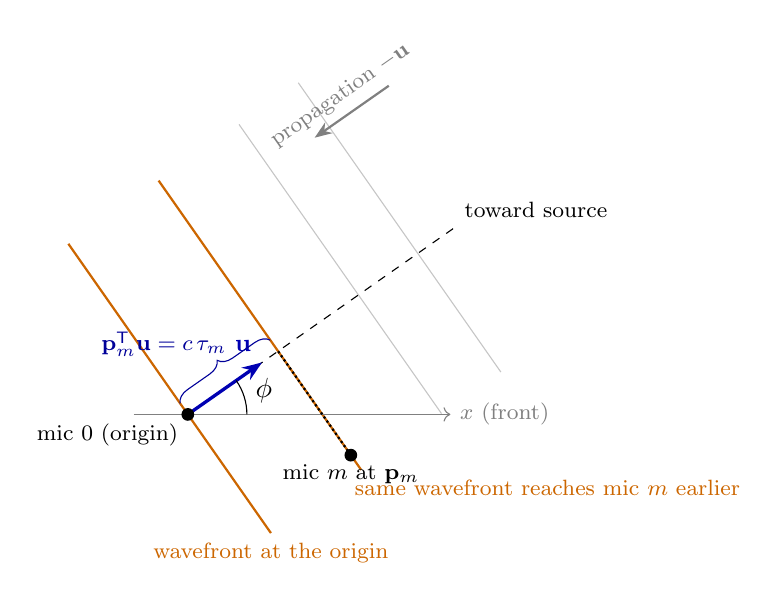
\begin{tikzpicture}[scale=1.15]
  \def\a{35}
  \coordinate (O) at (0,0);
  \coordinate (P) at (1.8,-0.45);
  \coordinate (X) at (1,0);
  \coordinate (U) at (\a:1);
  \coordinate (Q) at ($(O)!(P)!(\a:3)$);
  % generic wavefronts further upstream
  \foreach \s in {2.3,3.1}{
    \draw[gray!45] ($(\a:\s)+(\a+90:2.3)$) -- ($(\a:\s)+(\a-90:1.6)$);}
  % wavefronts through O and through P
  \draw[orange!80!black, thick] ($(O)+(\a+90:2.3)$) -- ($(O)+(\a-90:1.6)$)
        node[below, font=\footnotesize] {wavefront at the origin};
  \draw[orange!80!black, thick] ($(Q)+(\a+90:2.3)$) -- ($(Q)+(\a-90:1.6)$)
        node[below right, font=\footnotesize, xshift=-6pt] {same wavefront reaches mic $m$ earlier};
  % propagation arrow
  \draw[arr, gray] ($(\a:3.9)+(\a+90:1.7)$) -- ($(\a:2.9)+(\a+90:1.7)$)
        node[midway, above, sloped, font=\footnotesize] {propagation $-\vu$};
  % axes and direction
  \draw[->, gray] (-0.6,0) -- (2.9,0) node[right, font=\footnotesize] {$x$ (front)};
  \draw[dashed] (O) -- (\a:3.6) node[above right, font=\footnotesize] {toward source};
  \draw[-{Stealth[length=2.5mm]}, very thick, blue!70!black] (O) -- (U)
        node[above left, font=\small] {$\vu$};
  \pic[draw, "$\phi$", angle radius=0.75cm, angle eccentricity=1.35] {angle = X--O--U};
  % projection
  \draw[densely dotted, thick] (P) -- (Q);
  \draw[decorate, decoration={brace, amplitude=5pt}, blue!60!black]
        ($(O)+(\a+90:0.15)$) -- ($(Q)+(\a+90:0.15)$)
        node[midway, above left=2pt and -4pt, font=\footnotesize] {$\vp_m\tr\vu = c\,\tau_m$};
  \fill (O) circle (2pt) node[below left, font=\footnotesize] {mic 0 (origin)};
  \fill (P) circle (2pt) node[below, font=\footnotesize] {mic $m$ at $\vp_m$};
\end{tikzpicture}
\caption{A plane wave from azimuth $\phi$. Mic $m$ sits $\vp_m\tr\vu$ metres upstream of the
origin, so it hears the wave $\tau_m=\vp_m\tr\vu/c$ seconds earlier (lines~61--62).}
\label{fig:planewave}
\end{figure}

\paragraph{Derivation.}
Let $\vu=[\cos\phi,\ \sin\phi]\tr$ be the unit vector pointing \emph{toward} the source
(line~61). A plane wave that carries the signal $s(t)$ and travels in direction $-\vu$ has
pressure field
\begin{equation}
  p(\mathbf x,t)=s\!\left(t+\frac{\vu\tr\mathbf x}{c}\right).
\end{equation}
This is the right sign: points with $\vu\tr\mathbf x>0$ are closer to the source, so they see
a given part of $s$ earlier. Mic $m$ therefore records $x_m(t)=s(t+\tau_m)$, with
\begin{equation}\label{eq:tau}
  \tau_m=\frac{\vp_m\tr\vu}{c}\qquad\text{(line 62, \code{advance = positions @ direction / SPEED_OF_SOUND})}.
\end{equation}
NumPy's FFT uses the kernel $e^{-j2\pi ft}$. With that convention the shift theorem reads
$s(t+\tau)\;\longleftrightarrow\;e^{+j2\pi f\tau}S(f)$. Stacking the seven mics gives
\begin{equation}\label{eq:steer}
  \vx(f)=S(f)\,\vd(f,\phi),\qquad
  \vd(f,\phi)=\begin{bmatrix}e^{j2\pi f\tau_0}\\ \vdots\\ e^{j2\pi f\tau_6}\end{bmatrix}
  =\exp\!\big(j\kappa\,\vp_m\tr\vu\big)_{m=0}^{6}.
\end{equation}
The vector $\vd$ is the \emph{steering vector}: the array's fingerprint for direction $\phi$
at frequency $f$. All of its entries have modulus one, so $\|\vd\|^2=M$. Because $\vp_0=\mathbf 0$,
$d_0\equiv1$: the centre mic is the phase reference.

\demolines{58}{63}

\paragraph{Code map.} Line~63 evaluates \eqref{eq:steer} for every bin at once.
\code{freqs[:, None] * advance[None, :]} is the outer product $f_k\tau_m$, which gives an
$F\times M$ array with $F=N/2+1=257$ (\code{np.fft.rfftfreq(512, 1/48000)}, line~68,
returns $0, 93.75, \dots, 24\,000$\,Hz).

\paragraph{Assumptions, and when they hold.}
\begin{enumerate}
\item \emph{Far field.} The wavefronts are flat if the source distance $R$ satisfies the
  Fraunhofer criterion $R>2D^2/\lambda$. With $D=86$\,mm this is $0.17$\,m at 4\,kHz and
  even less at lower frequencies, so any talker further away than about an arm's length is
  in the far field.
\item \emph{In-plane, free-field propagation.} Elevation, scattering off the board and the
  mics' own responses are ignored. All mics are assumed identical and omnidirectional.
\item \emph{Multiplicative STFT model.} Equation~\eqref{eq:steer} is exact for the continuous
  Fourier transform. For an $N$-sample STFT frame it holds approximately as long as
  $|\tau_m|\ll N/f_s$. Here $\max|\tau_m|=125\,\mu\text{s}\approx6$ samples, compared with a
  frame of $512$ samples.
\end{enumerate}

% =============================================================================
\section{Distortionless beamforming and delay-and-sum}\label{sec:das}
% =============================================================================

A (narrowband) beamformer forms one output per bin as a linear combination of the mics:
\begin{equation}\label{eq:beam}
  Y(f)=\vw(f)\herm\vx(f)=\sum_{m=0}^{6}\overline{w_m(f)}\,X_m(f).
\end{equation}
The conjugate is a convention that makes $Y$ an inner product. The code follows it exactly:
\code{w_h = weights.conj()} (line~92) and \code{w[k].conj() @ d} (line~127).

\paragraph{Signal model and performance measures.}
Write each STFT bin as target plus noise, $\vx=S\vd+\vn$, with noise covariance
$\E[\vn\vn\herm]=\sigma_v^2\G$, where $\Gamma_{mm}=1$ (so $\G$ is a \emph{coherence}
matrix). Then
\begin{equation}
  Y=S\,(\vw\herm\vd)+\vw\herm\vn,\qquad
  \E|\vw\herm\vn|^2=\sigma_v^2\,\vw\herm\G\vw .
\end{equation}

\begin{definition}[Distortionless constraint; array gain]
A beamformer is \emph{distortionless} toward $\phi_0$ if $\vw\herm\vd(f,\phi_0)=1$ at every $f$.
Its \emph{array gain} against noise field $\G$ is the output SNR divided by the SNR at a single mic:
\begin{equation}\label{eq:gain}
  A_{\G}(\vw)=\frac{|\vw\herm\vd|^2}{\vw\herm\G\vw}.
\end{equation}
Two cases matter. The \emph{white-noise gain} is $\WNG=A_{\mI}$, for mic self-noise, which is
independent from mic to mic. The \emph{directivity index} is $\DI=A_{\G_{\mathrm{diff}}}$, for
reverberation and babble arriving from all directions (Section~\ref{sec:sd}).
\end{definition}

The distortionless constraint is why the talker's voice comes out with its original timbre.
Whatever happens to the noise, the target spectrum is multiplied by exactly~1 in every bin.

\demolines{72}{73}

\begin{proposition}[Delay-and-sum is the WNG-optimal distortionless beamformer]\label{prop:das}
Among all $\vw$ with $\vw\herm\vd=1$, the white-noise gain $1/\|\vw\|^2$ is maximised uniquely by
$\vw=\vd/M$ (line~73), and the maximum is $\WNG=M$, i.e.\ $10\log_{10}7=8.45$\,dB.
\end{proposition}
\begin{proof}
By Cauchy--Schwarz, $1=|\vw\herm\vd|^2\le\|\vw\|^2\|\vd\|^2=M\|\vw\|^2$, so
$\WNG=1/\|\vw\|^2\le M$. Equality holds iff $\vw\propto\vd$, and the constraint fixes the
constant: $\vw\herm\vd=\vd\herm\vd/M=1$.
\end{proof}

\begin{intuition}
$\overline{d_m}=e^{-j2\pi f\tau_m}$ undoes each mic's head start, so the seven copies of the
target line up and are averaged. Independent self-noise does not line up, so its power drops
by a factor of $M$.
\end{intuition}

\paragraph{Why delay-and-sum is not enough here.}
As $f\to0$, every steering vector tends to $\one$, whatever the direction. Then
$B(f,\phi)=\vd(f,0)\herm\vd(f,\phi)/M\to1$ for all $\phi$, and the array is omnidirectional.
Quantitatively, at 281\,Hz the wavelength is $1.22$\,m, fourteen times the aperture.
DAS's directivity index there is only $0.15$\,dB (Figure~\ref{fig:wngdi}), while most of the
energy in speech and room noise lies below 1\,kHz. Getting directivity out of a small array
needs a different criterion.

% =============================================================================
\section{Superdirective (MVDR) beamforming against diffuse noise}\label{sec:sd}
% =============================================================================

\subsection{The diffuse noise field}

Reverberation and distant babble behave like a \emph{spherically isotropic} (diffuse) field:
infinitely many mutually uncorrelated plane waves of equal power, arriving uniformly from all
directions in 3-D.

\begin{proposition}[Diffuse-field coherence]\label{prop:sinc}
In a diffuse field, the coherence between two omnidirectional mics a distance $d_{ij}$ apart is
\begin{equation}\label{eq:sinc}
  \Gamma_{ij}(f)=\frac{\sin(\kappa d_{ij})}{\kappa d_{ij}},\qquad \kappa=\frac{2\pi f}{c}.
\end{equation}
\end{proposition}
\begin{proof}
Each plane wave from direction $\vu\in S^2$ contributes $e^{j\kappa\vu\tr\vp_i}$ to mic $i$.
The waves are uncorrelated and have equal power, so
\[
  \Gamma_{ij}=\frac{1}{4\pi}\oint_{S^2}e^{j\kappa\,\vu\tr(\vp_i-\vp_j)}\,d\Omega(\vu).
\]
Choose the polar axis along $\vp_i-\vp_j$, so that $\vu\tr(\vp_i-\vp_j)=d_{ij}\cos\vartheta$.
The azimuthal integral contributes $2\pi$. Substituting $\mu=\cos\vartheta$,
\[
  \Gamma_{ij}=\frac{1}{2}\int_0^{\pi}e^{j\kappa d_{ij}\cos\vartheta}\sin\vartheta\,d\vartheta
  =\frac12\int_{-1}^{1}e^{j\kappa d_{ij}\mu}\,d\mu=\frac{\sin(\kappa d_{ij})}{\kappa d_{ij}}.\qedhere
\]
\end{proof}

NumPy's \code{np.sinc(x)} is the \emph{normalised} sinc, $\sin(\pi x)/(\pi x)$. With
$x=2fd/c$ we get $\pi x=2\pi f d/c=\kappa d$, so line~79 is exactly~\eqref{eq:sinc}.
\code{dist} (line~76) holds the $7\times7$ matrix of $d_{ij}$, and its diagonal gives
$\Gamma_{ii}=\operatorname{sinc}(0)=1$.

\begin{remark}
The array is planar, but room noise is three-dimensional, so the 3-D (spherical) average is the
right model. A purely 2-D (cylindrical) field would give $J_0(\kappa d)$ instead.
\end{remark}

\begin{figure}[ht]
\centering
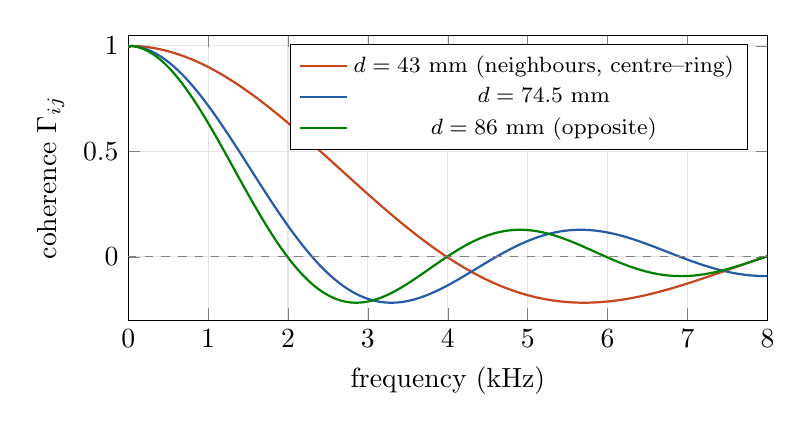
\begin{tikzpicture}
\begin{axis}[width=0.8\linewidth, height=5.2cm, xmin=0, xmax=8, ymin=-0.3, ymax=1.05,
  xlabel={frequency (kHz)}, ylabel={coherence $\Gamma_{ij}$}, grid=major, grid style={gray!20},
  legend pos=north east, legend style={font=\footnotesize}, samples=200]
  \addplot[thick, sdcol, domain=0.001:8] {sin(deg(0.78770*x))/(0.78770*x)};
  \addlegendentry{$d=43$ mm (neighbours, centre--ring)}
  \addplot[thick, dascol, domain=0.001:8] {sin(deg(1.36434*x))/(1.36434*x)};
  \addlegendentry{$d=74.5$ mm}
  \addplot[thick, green!50!black, domain=0.001:8] {sin(deg(1.57540*x))/(1.57540*x)};
  \addlegendentry{$d=86$ mm (opposite)}
  \addplot[gray, dashed, domain=0:8] {0};
\end{axis}
\end{tikzpicture}
\caption{Diffuse-noise coherence \eqref{eq:sinc} for the three spacings of
Proposition~\ref{prop:dist}. Below about 1\,kHz every pair is almost perfectly coherent.}
\label{fig:coherence}
\end{figure}

\begin{intuition}
Below about 1\,kHz, every pair of mics hears nearly the \emph{same} diffuse noise
(Figure~\ref{fig:coherence}). Noise that is common to all mics can be removed by
\emph{subtracting} them, much as a differential (gradient) microphone does. A sound from the
front is not identical at all mics, because it carries the small phase slope $\vd$. So a
carefully chosen set of differences can cancel most of the diffuse field and still pass the
target. The price is that differencing nearly identical signals amplifies anything that is
\emph{not} common, in particular each mic's own self-noise. That trade-off is the whole story of
diagonal loading below.
\end{intuition}

\subsection{The optimal weights}

\begin{proposition}[MVDR / superdirective solution]\label{prop:mvdr}
Let $\Gmu=\G+\mu\mI$ with $\mu>0$. The problem
\begin{equation}
  \min_{\vw}\ \vw\herm\Gmu\vw\quad\text{subject to}\quad \vw\herm\vd=1
\end{equation}
has the unique solution
\begin{equation}\label{eq:mvdr}
  \boxed{\ \vw=\frac{\Gmu^{-1}\vd}{\vd\herm\Gmu^{-1}\vd}\ }
  \qquad\text{with minimum value}\qquad \frac{1}{\vd\herm\Gmu^{-1}\vd}.
\end{equation}
\end{proposition}
\begin{proof}
$\G$ is an average of rank-one matrices $\mathbf a\mathbf a\herm$ (see the proof of
Proposition~\ref{prop:sinc}), so it is Hermitian positive semidefinite. Hence $\Gmu$ is
positive definite and has a positive-definite square root. Apply Cauchy--Schwarz to the
vectors $\Gmu^{1/2}\vw$ and $\Gmu^{-1/2}\vd$:
\[
  1=|\vw\herm\vd|^2=\big|(\Gmu^{1/2}\vw)\herm(\Gmu^{-1/2}\vd)\big|^2
  \le(\vw\herm\Gmu\vw)\,(\vd\herm\Gmu^{-1}\vd).
\]
So $\vw\herm\Gmu\vw\ge1/(\vd\herm\Gmu^{-1}\vd)$, with equality iff
$\Gmu^{1/2}\vw\propto\Gmu^{-1/2}\vd$, i.e.\ $\vw\propto\Gmu^{-1}\vd$. The constraint fixes the
scale and gives \eqref{eq:mvdr}.
\end{proof}

This is the same argument as Proposition~\ref{prop:das}, carried out in the inner product
weighted by $\Gmu$. Delay-and-sum is simply the special case $\Gmu=\mI$.

\demolines{75}{82}

\paragraph{Code map.} Line~79 builds $\Gmu(f_k)$. Line~80 computes $\Gmu^{-1}\vd$ by solving the
linear system rather than forming an inverse, which is cheaper and numerically more accurate.
Line~81 divides by $\vd\herm\Gmu^{-1}\vd$, a real positive scalar because $\Gmu^{-1}$ is
Hermitian positive definite. The loop runs 257 small $7\times7$ solves, \emph{once}, at
start-up (line~197). The real-time callback never touches this code.

\subsection{Why the diagonal loading is essential}\label{sec:loading}

\paragraph{Ill-conditioning at low frequency.} As $f\to0$, \eqref{eq:sinc} gives
$\G\to\one\one\tr$, a rank-one matrix, so $\G^{-1}$ blows up. The condition numbers of the
actual $7\times7$ matrices (computed from the code's geometry) are:

\begin{center}\small
\begin{tabular}{@{}lcccc@{}}
\toprule
$f$ & 100 Hz & 300 Hz & 1 kHz & 3 kHz\\
\midrule
$\operatorname{cond}(\G)$ & $1.2\times10^{10}$ & $1.7\times10^{7}$ & $1.1\times10^{4}$ & $7.8$\\
$\operatorname{cond}(\G+0.05\,\mI)$ & $141$ & $139$ & $117$ & $6.6$\\
\bottomrule
\end{tabular}
\end{center}

\noindent
Without loading, the unconstrained weights at 100\,Hz would be huge and of alternating sign.
They would cancel the diffuse field perfectly \emph{on paper}, but they would amplify mic
self-noise by the factor $\|\vw\|^2=1/\WNG$, which is enormous.

\paragraph{Three equivalent readings of $\mu$.}
\begin{enumerate}
\item \emph{Tikhonov regularisation.} $\vw\herm\Gmu\vw=\vw\herm\G\vw+\mu\|\vw\|^2$. The
  objective adds a penalty on the weight norm, i.e.\ on self-noise amplification, to the
  diffuse-noise power.
\item \emph{A physical noise model.} $\Gmu$ is the coherence of diffuse noise plus uncorrelated
  sensor noise whose power is $\mu$ times the diffuse power. The design is optimal for that mixed
  field.
\item \emph{A dial between two designs.} At $\mu\to0$ the design is fully superdirective. As
  $\mu\to\infty$ it becomes delay-and-sum. To see the second limit, expand
  $\Gmu^{-1}=\mu^{-1}(\mI+\G/\mu)^{-1}=\mu^{-1}\big(\mI-\G/\mu+O(\mu^{-2})\big)$. Then
  $\Gmu^{-1}\vd\propto\vd+O(\mu^{-1})$, and after normalising, $\vw\to\vd/M$.
\end{enumerate}

\paragraph{The measured trade-off.} The table sweeps $\mu$ at the 281\,Hz bin, using the
code's geometry. WNG and DI are defined in~\eqref{eq:gain}, and ``back'' is $|B|$ at
$\phi=180^\circ$.

\begin{center}\small
\begin{tabular}{@{}lcccccc@{}}
\toprule
$\mu$ & 0.001 & 0.01 & \textbf{0.05 (used)} & 0.2 & 1 & 10\\
\midrule
WNG (dB) & $-13.6$ & $-5.8$ & $\mathbf{-4.0}$ & $-0.2$ & $+6.2$ & $+8.4$\\
DI (dB)  & $6.8$ & $6.1$ & $\mathbf{5.5}$ & $3.6$ & $1.2$ & $0.3$\\
back (dB) & $-9.1$ & $-7.7$ & $\mathbf{-14.2}$ & $-12.2$ & $-2.8$ & $-0.6$\\
$\max_m|w_m|$ & 2.42 & 0.94 & \textbf{0.78} & 0.50 & 0.22 & 0.14\\
\bottomrule
\end{tabular}
\end{center}

\begin{rationale}[: \texttt{DIAGONAL\_LOADING = 0.05}]
At $\mu=0.05$ the 281\,Hz beam gains $5.4$\,dB of directivity over delay-and-sum ($5.5$ vs
$0.15$\,dB). In exchange, mic self-noise is $4$\,dB \emph{louder} than with a single mic, and
$12.4$\,dB louder than with DAS. Going down to $\mu=0.001$ buys only $1.3$\,dB more DI and costs
almost $10$\,dB more hiss. Going up to $\mu=1$ throws most of the directivity away. So $0.05$
sits near the knee of the curve. The deep rear null at $0.05$ is a helpful side effect of
where the null lands, not something the criterion optimises. If the output hisses in a quiet
room, raise $\mu$. If it sounds roomy, lower it.
\end{rationale}

\paragraph{Limiting cases that check the code.}
\begin{itemize}
\item \emph{DC bin} ($f=0$): $\vd=\one$ and $\Gmu=\one\one\tr+\mu\mI$. Since
  $\Gmu\one=(M+\mu)\one$, we get $\Gmu^{-1}\one=\one/(M+\mu)$ and therefore $\vw=\one/M$:
  exactly delay-and-sum.
\item \emph{High frequency}: the off-diagonal entries of $\G$ decay like $1/(\kappa d)$, so
  $\G\to\mI$ and the superdirective weights tend to DAS. This is visible in
  Figure~\ref{fig:wngdi}: the curves merge above roughly 3.5\,kHz, where
  $\operatorname{cond}(\G)$ is already below 8.
\end{itemize}

% =============================================================================
\section{Beam pattern, white-noise gain and spatial aliasing}\label{sec:pattern}
% =============================================================================

\begin{definition}[Beam pattern]
For weights designed toward $\phi_0$, the response to a unit plane wave from $\phi$ is
\begin{equation}
  B(f,\phi)=\vw(f)\herm\vd(f,\phi),\qquad B_{\mathrm{dB}}=20\log_{10}|B|.
\end{equation}
The distortionless constraint gives $B(f,\phi_0)=1=0$\,dB.
\end{definition}

\demolines{112}{131}

\paragraph{Code map.} Line~126 builds $\vd(f_k,\phi_0+\phi)$ for each test azimuth. Line~127
evaluates $20\log_{10}|\vw\herm\vd|$; the \code{1e-12} keeps $\log 0$ away at exact nulls.
Line~128 is $\WNG=1/\|\vw\|^2$, which is valid because $|\vw\herm\vd|=1$. Line~123 rounds each
requested frequency to the nearest bin, which is why the printout shows 281\,Hz rather than 250.

\begin{figure}[p]
\centering
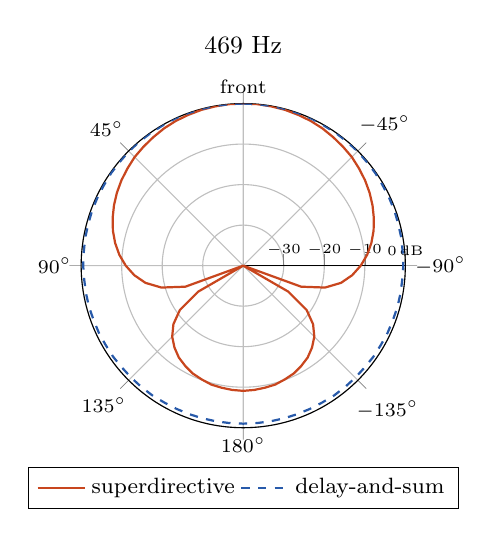
\begin{tikzpicture}
\begin{polaraxis}[width=0.47\linewidth, title={\small 469 Hz}, ymin=0, ymax=40,
  ytick={10,20,30,40}, yticklabels={$-30$,$-20$,$-10$,$0$\,dB}, yticklabel style={font=\tiny},
  xtick={0,45,...,315}, xticklabel style={font=\scriptsize},
  xticklabels={$-90^\circ$,$-45^\circ$,front,$45^\circ$,$90^\circ$,$135^\circ$,$180^\circ$,$-135^\circ$},
  x filter/.expression={x+90}, y filter/.expression={y+40},
  legend style={at={(0.5,-0.12)}, anchor=north, font=\footnotesize, legend columns=2}]
\addplot[thick, sdcol, no markers] coordinates {(0,0.0) (5,-0.0) (10,-0.1) (15,-0.2) (20,-0.4) (25,-0.6) (30,-0.9) (35,-1.3) (40,-1.7) (45,-2.1) (50,-2.7) (55,-3.3) (60,-4.0) (65,-4.8) (70,-5.7) (75,-6.7) (80,-7.9) (85,-9.3) (90,-11.0) (95,-13.0) (100,-15.5) (105,-19.1) (110,-24.8) (115,-40.0) (120,-27.2) (125,-20.9) (130,-17.5) (135,-15.2) (140,-13.6) (145,-12.3) (150,-11.4) (155,-10.6) (160,-10.1) (165,-9.6) (170,-9.4) (175,-9.2) (180,-9.1) (185,-9.2) (190,-9.4) (195,-9.6) (200,-10.1) (205,-10.6) (210,-11.4) (215,-12.3) (220,-13.6) (225,-15.2) (230,-17.5) (235,-20.9) (240,-27.2) (245,-40.0) (250,-24.8) (255,-19.1) (260,-15.5) (265,-13.0) (270,-11.0) (275,-9.3) (280,-7.9) (285,-6.7) (290,-5.7) (295,-4.8) (300,-4.0) (305,-3.3) (310,-2.7) (315,-2.1) (320,-1.7) (325,-1.3) (330,-0.9) (335,-0.6) (340,-0.4) (345,-0.2) (350,-0.1) (355,-0.0) (360,0.0)};
\addlegendentry{superdirective}
\addplot[thick, dascol, dashed, no markers] coordinates {(0,0.0) (5,-0.0) (10,-0.0) (15,-0.0) (20,-0.0) (25,-0.0) (30,-0.1) (35,-0.1) (40,-0.1) (45,-0.1) (50,-0.2) (55,-0.2) (60,-0.3) (65,-0.3) (70,-0.3) (75,-0.4) (80,-0.4) (85,-0.5) (90,-0.5) (95,-0.6) (100,-0.6) (105,-0.6) (110,-0.7) (115,-0.7) (120,-0.8) (125,-0.8) (130,-0.9) (135,-0.9) (140,-0.9) (145,-0.9) (150,-1.0) (155,-1.0) (160,-1.0) (165,-1.0) (170,-1.0) (175,-1.0) (180,-1.0) (185,-1.0) (190,-1.0) (195,-1.0) (200,-1.0) (205,-1.0) (210,-1.0) (215,-0.9) (220,-0.9) (225,-0.9) (230,-0.9) (235,-0.8) (240,-0.8) (245,-0.7) (250,-0.7) (255,-0.6) (260,-0.6) (265,-0.6) (270,-0.5) (275,-0.5) (280,-0.4) (285,-0.4) (290,-0.3) (295,-0.3) (300,-0.3) (305,-0.2) (310,-0.2) (315,-0.1) (320,-0.1) (325,-0.1) (330,-0.1) (335,-0.0) (340,-0.0) (345,-0.0) (350,-0.0) (355,-0.0) (360,0.0)};
\addlegendentry{delay-and-sum}
\end{polaraxis}
\end{tikzpicture}\hfill
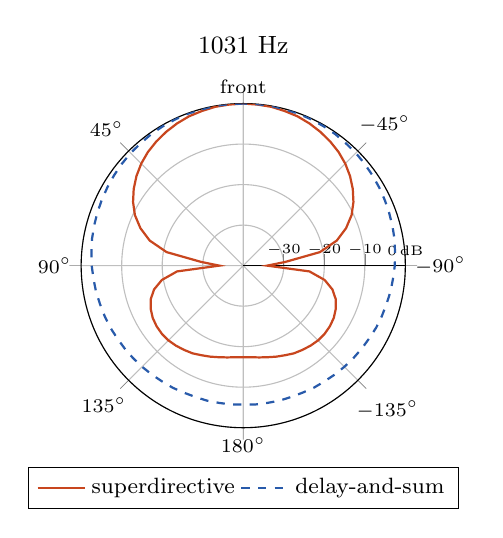
\begin{tikzpicture}
\begin{polaraxis}[width=0.47\linewidth, title={\small 1031 Hz}, ymin=0, ymax=40,
  ytick={10,20,30,40}, yticklabels={$-30$,$-20$,$-10$,$0$\,dB}, yticklabel style={font=\tiny},
  xtick={0,45,...,315}, xticklabel style={font=\scriptsize},
  xticklabels={$-90^\circ$,$-45^\circ$,front,$45^\circ$,$90^\circ$,$135^\circ$,$180^\circ$,$-135^\circ$},
  x filter/.expression={x+90}, y filter/.expression={y+40},
  legend style={at={(0.5,-0.12)}, anchor=north, font=\footnotesize, legend columns=2}]
\addplot[thick, sdcol, no markers] coordinates {(0,0.0) (5,-0.1) (10,-0.2) (15,-0.5) (20,-0.8) (25,-1.3) (30,-1.9) (35,-2.6) (40,-3.4) (45,-4.4) (50,-5.6) (55,-7.0) (60,-8.6) (65,-10.5) (70,-13.0) (75,-16.1) (80,-20.8) (85,-29.6) (90,-34.1) (95,-23.6) (100,-19.6) (105,-17.2) (110,-15.7) (115,-14.8) (120,-14.2) (125,-13.9) (130,-13.8) (135,-13.9) (140,-14.2) (145,-14.6) (150,-15.0) (155,-15.6) (160,-16.1) (165,-16.6) (170,-17.0) (175,-17.3) (180,-17.4) (185,-17.3) (190,-17.0) (195,-16.6) (200,-16.1) (205,-15.6) (210,-15.0) (215,-14.6) (220,-14.2) (225,-13.9) (230,-13.8) (235,-13.9) (240,-14.2) (245,-14.8) (250,-15.7) (255,-17.2) (260,-19.6) (265,-23.6) (270,-34.1) (275,-29.6) (280,-20.8) (285,-16.1) (290,-13.0) (295,-10.5) (300,-8.6) (305,-7.0) (310,-5.6) (315,-4.4) (320,-3.4) (325,-2.6) (330,-1.9) (335,-1.3) (340,-0.8) (345,-0.5) (350,-0.2) (355,-0.1) (360,0.0)};
\addlegendentry{superdirective}
\addplot[thick, dascol, dashed, no markers] coordinates {(0,0.0) (5,-0.0) (10,-0.0) (15,-0.1) (20,-0.1) (25,-0.2) (30,-0.3) (35,-0.4) (40,-0.6) (45,-0.7) (50,-0.9) (55,-1.1) (60,-1.3) (65,-1.5) (70,-1.7) (75,-1.9) (80,-2.1) (85,-2.4) (90,-2.6) (95,-2.9) (100,-3.1) (105,-3.4) (110,-3.6) (115,-3.8) (120,-4.1) (125,-4.3) (130,-4.5) (135,-4.7) (140,-4.9) (145,-5.1) (150,-5.2) (155,-5.4) (160,-5.5) (165,-5.5) (170,-5.6) (175,-5.6) (180,-5.7) (185,-5.6) (190,-5.6) (195,-5.5) (200,-5.5) (205,-5.4) (210,-5.2) (215,-5.1) (220,-4.9) (225,-4.7) (230,-4.5) (235,-4.3) (240,-4.1) (245,-3.8) (250,-3.6) (255,-3.4) (260,-3.1) (265,-2.9) (270,-2.6) (275,-2.4) (280,-2.1) (285,-1.9) (290,-1.7) (295,-1.5) (300,-1.3) (305,-1.1) (310,-0.9) (315,-0.7) (320,-0.6) (325,-0.4) (330,-0.3) (335,-0.2) (340,-0.1) (345,-0.1) (350,-0.0) (355,-0.0) (360,0.0)};
\addlegendentry{delay-and-sum}
\end{polaraxis}
\end{tikzpicture}

\vspace{6pt}
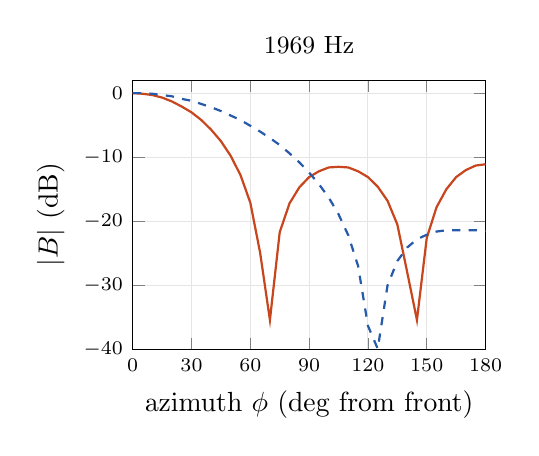
\begin{tikzpicture}
\begin{axis}[width=0.5\linewidth, height=5cm, title={\small 1969 Hz}, xmin=0, xmax=180,
  ymin=-40, ymax=2, xtick={0,30,...,180}, xlabel={azimuth $\phi$ (deg from front)},
  ylabel={$|B|$ (dB)}, grid=major, grid style={gray!20}, tick label style={font=\scriptsize}]
\addplot[thick, sdcol, no markers] coordinates {(0,0.0) (5,-0.1) (10,-0.3) (15,-0.7) (20,-1.3) (25,-2.1) (30,-3.0) (35,-4.2) (40,-5.7) (45,-7.5) (50,-9.8) (55,-12.8) (60,-17.1) (65,-24.9) (70,-35.4) (75,-21.7) (80,-17.2) (85,-14.7) (90,-13.1) (95,-12.2) (100,-11.6) (105,-11.5) (110,-11.6) (115,-12.2) (120,-13.1) (125,-14.6) (130,-16.8) (135,-20.5) (140,-27.9) (145,-35.4) (150,-22.6) (155,-17.8) (160,-15.0) (165,-13.1) (170,-12.0) (175,-11.3) (180,-11.1)};
\addplot[thick, dascol, dashed, no markers] coordinates {(0,0.0) (5,-0.0) (10,-0.1) (15,-0.3) (20,-0.5) (25,-0.9) (30,-1.2) (35,-1.7) (40,-2.2) (45,-2.8) (50,-3.5) (55,-4.2) (60,-5.1) (65,-6.0) (70,-7.0) (75,-8.1) (80,-9.4) (85,-10.8) (90,-12.4) (95,-14.2) (100,-16.3) (105,-18.9) (110,-22.2) (115,-27.0) (120,-36.3) (125,-39.9) (130,-30.0) (135,-26.2) (140,-24.1) (145,-22.8) (150,-22.1) (155,-21.6) (160,-21.4) (165,-21.4) (170,-21.4) (175,-21.4) (180,-21.5)};
\end{axis}
\end{tikzpicture}\hfill
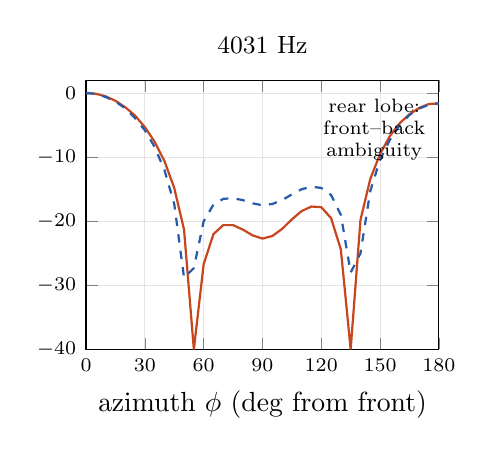
\begin{tikzpicture}
\begin{axis}[width=0.5\linewidth, height=5cm, title={\small 4031 Hz}, xmin=0, xmax=180,
  ymin=-40, ymax=2, xtick={0,30,...,180}, xlabel={azimuth $\phi$ (deg from front)},
  grid=major, grid style={gray!20}, tick label style={font=\scriptsize}]
\addplot[thick, sdcol, no markers] coordinates {(0,0.0) (5,-0.1) (10,-0.5) (15,-1.2) (20,-2.2) (25,-3.5) (30,-5.3) (35,-7.6) (40,-10.6) (45,-14.8) (50,-21.3) (55,-40.0) (60,-26.7) (65,-22.0) (70,-20.6) (75,-20.6) (80,-21.3) (85,-22.2) (90,-22.7) (95,-22.3) (100,-21.2) (105,-19.7) (110,-18.4) (115,-17.7) (120,-17.8) (125,-19.5) (130,-24.4) (135,-40.0) (140,-19.8) (145,-13.4) (150,-9.5) (155,-6.7) (160,-4.7) (165,-3.3) (170,-2.3) (175,-1.7) (180,-1.6)};
\addplot[thick, dascol, dashed, no markers] coordinates {(0,0.0) (5,-0.1) (10,-0.6) (15,-1.3) (20,-2.4) (25,-3.9) (30,-5.8) (35,-8.4) (40,-12.0) (45,-17.3) (50,-28.8) (55,-27.3) (60,-20.0) (65,-17.4) (70,-16.5) (75,-16.4) (80,-16.7) (85,-17.2) (90,-17.5) (95,-17.3) (100,-16.7) (105,-15.8) (110,-15.0) (115,-14.6) (120,-14.8) (125,-15.9) (130,-19.0) (135,-28.0) (140,-25.0) (145,-15.3) (150,-10.4) (155,-7.3) (160,-5.0) (165,-3.4) (170,-2.4) (175,-1.8) (180,-1.6)};
\node[font=\scriptsize, align=center, anchor=south east] at (axis cs:178,-12) {rear lobe:\\front--back\\ambiguity};
\end{axis}
\end{tikzpicture}
\caption{Beam patterns computed from \texttt{design\_weights} (5$^\circ$ grid, values floored at
$-40$\,dB). Solid: superdirective ($\mu=0.05$); dashed: delay-and-sum. In the polar plots the
front is at the top and the left at the left. The bottom plots show only $0$--$180^\circ$,
which is enough by Proposition~\ref{prop:symmetry}.}
\label{fig:patterns}
\end{figure}

\paragraph{Reading the patterns.} Half-width at $-3$\,dB, read off the 5$^\circ$ grid:

\begin{center}\small
\begin{tabular}{@{}lcccc@{}}
\toprule
& 469 Hz & 1031 Hz & 1969 Hz & 4031 Hz\\
\midrule
superdirective & $\approx53^\circ$ & $\approx37^\circ$ & $\approx30^\circ$ & $\approx23^\circ$\\
delay-and-sum  & none (min $-1.0$\,dB) & $\approx97^\circ$ & $\approx46^\circ$ & $\approx22^\circ$\\
\bottomrule
\end{tabular}
\end{center}

\noindent
Below 2\,kHz the superdirective design gives a genuine forward lobe where delay-and-sum is nearly
omnidirectional. Above 4\,kHz the two are essentially the same, as predicted in
Section~\ref{sec:loading}.

\begin{figure}[ht]
\centering
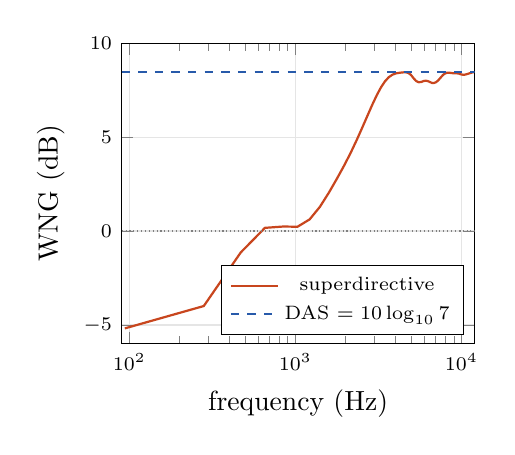
\begin{tikzpicture}
\begin{axis}[width=0.5\linewidth, height=5.4cm, xmode=log, xmin=90, xmax=12000,
  ymin=-6, ymax=10, xlabel={frequency (Hz)}, ylabel={WNG (dB)}, grid=major, grid style={gray!20},
  legend pos=south east, legend style={font=\scriptsize}, tick label style={font=\scriptsize}]
\addplot[thick, sdcol, no markers] coordinates {(94,-5.18) (281,-3.99) (469,-1.14) (656,0.17) (844,0.24) (1031,0.23) (1219,0.62) (1406,1.29) (1594,2.05) (1781,2.79) (1969,3.49) (2156,4.17) (2344,4.85) (2531,5.51) (2719,6.14) (2906,6.72) (3094,7.23) (3281,7.65) (3469,7.97) (3656,8.19) (3844,8.32) (4031,8.39) (4219,8.42) (4406,8.44) (4594,8.45) (4781,8.42) (4969,8.31) (5156,8.13) (5344,7.98) (5531,7.92) (5719,7.93) (5906,7.98) (6094,8.00) (6281,7.98) (6469,7.93) (6656,7.88) (6844,7.88) (7031,7.92) (7219,8.00) (7406,8.11) (7594,8.22) (7781,8.32) (7969,8.38) (8156,8.42) (8344,8.42) (8531,8.42) (8719,8.41) (8906,8.40) (9094,8.40) (9281,8.40) (9469,8.39) (9656,8.38) (9844,8.35) (10031,8.33) (10219,8.32) (10406,8.32) (10594,8.33) (10781,8.35) (10969,8.37) (11156,8.39) (11344,8.41) (11531,8.43) (11719,8.45) (11906,8.45)};
\addlegendentry{superdirective}
\addplot[thick, dascol, dashed, domain=90:12000] {8.45};
\addlegendentry{DAS $=10\log_{10}7$}
\addplot[gray, densely dotted, domain=90:12000] {0};
\end{axis}
\end{tikzpicture}\hfill
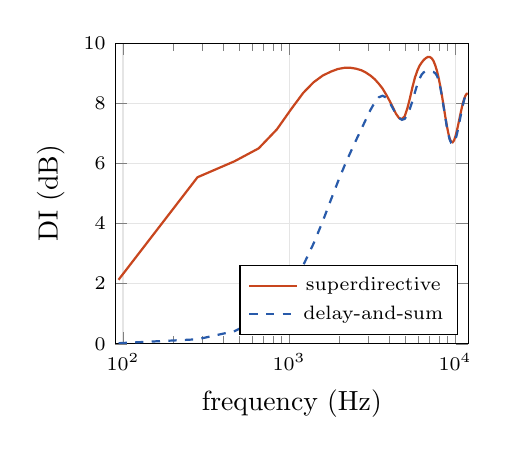
\begin{tikzpicture}
\begin{axis}[width=0.5\linewidth, height=5.4cm, xmode=log, xmin=90, xmax=12000,
  ymin=0, ymax=10, xlabel={frequency (Hz)}, ylabel={DI (dB)}, grid=major, grid style={gray!20},
  legend pos=south east, legend style={font=\scriptsize}, tick label style={font=\scriptsize}]
\addplot[thick, sdcol, no markers] coordinates {(94,2.13) (281,5.54) (469,6.07) (656,6.50) (844,7.13) (1031,7.81) (1219,8.35) (1406,8.70) (1594,8.92) (1781,9.05) (1969,9.14) (2156,9.18) (2344,9.18) (2531,9.15) (2719,9.10) (2906,9.02) (3094,8.92) (3281,8.80) (3469,8.65) (3656,8.49) (3844,8.29) (4031,8.08) (4219,7.86) (4406,7.65) (4594,7.51) (4781,7.47) (4969,7.57) (5156,7.83) (5344,8.17) (5531,8.53) (5719,8.84) (5906,9.07) (6094,9.24) (6281,9.35) (6469,9.44) (6656,9.50) (6844,9.54) (7031,9.54) (7219,9.50) (7406,9.41) (7594,9.26) (7781,9.07) (7969,8.83) (8156,8.54) (8344,8.23) (8531,7.90) (8719,7.57) (8906,7.27) (9094,7.01) (9281,6.82) (9469,6.72) (9656,6.70) (9844,6.76) (10031,6.89) (10219,7.06) (10406,7.25) (10594,7.46) (10781,7.66) (10969,7.85) (11156,8.02) (11344,8.15) (11531,8.25) (11719,8.31) (11906,8.33)};
\addlegendentry{superdirective}
\addplot[thick, dascol, dashed, no markers] coordinates {(94,0.02) (281,0.15) (469,0.42) (656,0.81) (844,1.32) (1031,1.93) (1219,2.62) (1406,3.34) (1594,4.07) (1781,4.77) (1969,5.39) (2156,5.92) (2344,6.37) (2531,6.77) (2719,7.13) (2906,7.47) (3094,7.78) (3281,8.03) (3469,8.20) (3656,8.25) (3844,8.19) (4031,8.03) (4219,7.83) (4406,7.64) (4594,7.51) (4781,7.45) (4969,7.48) (5156,7.61) (5344,7.82) (5531,8.07) (5719,8.35) (5906,8.61) (6094,8.81) (6281,8.95) (6469,9.03) (6656,9.06) (6844,9.06) (7031,9.06) (7219,9.05) (7406,9.04) (7594,9.00) (7781,8.91) (7969,8.75) (8156,8.51) (8344,8.21) (8531,7.87) (8719,7.54) (8906,7.23) (9094,6.98) (9281,6.79) (9469,6.68) (9656,6.65) (9844,6.69) (10031,6.79) (10219,6.94) (10406,7.13) (10594,7.35) (10781,7.56) (10969,7.77) (11156,7.96) (11344,8.12) (11531,8.25) (11719,8.30) (11906,8.33)};
\addlegendentry{delay-and-sum}
\end{axis}
\end{tikzpicture}
\caption{The core trade-off, computed for every other bin. Left: white-noise gain. Below about
600\,Hz the superdirective beam \emph{amplifies} self-noise relative to one mic (WNG $<0$\,dB);
this is the hiss that \code{DIAGONAL_LOADING} controls. Right: directivity index against diffuse
noise (computed with the unloaded $\G$). At 281\,Hz the superdirective design has 5.5\,dB, where
DAS has 0.15\,dB.}
\label{fig:wngdi}
\end{figure}

\subsection{Spatial aliasing and the front--back lobe}

A uniformly sampled line array obeys a \emph{spatial} Nyquist rule: the spacing must be below
$\lambda/2$, i.e.\ $f<c/(2d_{\min})=343/(2\cdot0.043)\approx3.99$\,kHz. A hexagon is not a
line, but the same mechanism gives one clean, exact result.

\begin{proposition}[Front/back ambiguity at 4.61 kHz]
At $f^\star=c/(2r\cos30^\circ)\approx4.61$\,kHz, the steering vectors for $\phi=0^\circ$ and
$\phi=180^\circ$ are identical. Every beamformer then has $|B(f^\star,180^\circ)|=|B(f^\star,0^\circ)|=1$.
\end{proposition}
\begin{proof}
For $\phi=0^\circ$ and $180^\circ$, $\vu=\pm\mathbf e_x$, so $d_m=e^{\pm j\kappa x_m}$, where
$x_m$ is mic $m$'s front coordinate. The two vectors agree iff $e^{2j\kappa x_m}=1$ for all
$m$. The $x_m$ take the values $0$ (mics 0, 1, 4) and $\pm r\cos30^\circ=\pm37.2$\,mm (mics
5, 6, 2, 3). So the condition is $2\kappa\cdot37.2\,\text{mm}\in2\pi\mathbb Z$, whose smallest
positive solution is $f^\star=c/(2\cdot0.0372)$.
\end{proof}

The 4031\,Hz panel of Figure~\ref{fig:patterns} is already approaching $f^\star$, and shows a
$-1.6$\,dB lobe straight behind the array for \emph{both} designs. No choice of weights can fix
this, because it is a property of the geometry. In practice the array gives useful rejection
from about 300\,Hz to 4\,kHz, which covers most of the energy and intelligibility of speech.

% =============================================================================
\section{Streaming: STFT analysis, beamforming, overlap-add synthesis}\label{sec:stft}
% =============================================================================

\demolines{85}{109}

\subsection{What one call to \texttt{process} computes}

Index blocks so that block $t$ holds samples $[tH,(t+1)H)$. When block $t$ arrives,
\code{in_buf} holds frame $t$, the $N=2H$ samples $x_m[(t-1)H+n]$ for $n=0,\dots,N-1$
(lines~98--99). Let $g[n]$ be the window. The algorithm is:
\begin{align}
  X_m^{(t)}[k]&=\sum_{n=0}^{N-1}g[n]\,x_m[(t-1)H+n]\,e^{-j2\pi kn/N}
     &&\text{(analysis, line 101)}\\
  Y^{(t)}[k]&=\sum_{m}\overline{w_{k,m}}\,X_m^{(t)}[k]=\vw_k\herm\vx^{(t)}[k]
     &&\text{(beamform, line 102)}\\
  y^{(t)}[n]&=g[n]\cdot\frac1N\sum_{k=0}^{N-1}Y^{(t)}[k]\,e^{j2\pi kn/N}
     &&\text{(synthesis, line 103)}\\
  y[(t-1)H+n]&\mathrel{+}=y^{(t)}[n]
     &&\text{(overlap-add, line 105)}
\end{align}
In the synthesis line, \code{irfft} fills in the bins $k>N/2$ by Hermitian symmetry,
$Y[N-k]=\overline{Y[k]}$, which guarantees a real output. Equivalently, the weights define
real-valued filters.

The \code{einsum("fm,fm->f", ...)} on line~102 multiplies the two $257\times7$ arrays
element-wise and sums over the mic index: 257 independent 7-term dot products. It never forms
a $257\times257$ matrix, which \code{w_h @ spec} would.

\subsection{The window and perfect reconstruction}

Line~91 builds $g[n]=\sqrt{h[n]}$ from the \emph{periodic} Hann window:
\begin{equation}
  h[n]=\tfrac12-\tfrac12\cos\!\frac{2\pi n}{N}=\sin^2\!\frac{\pi n}{N},
  \qquad g[n]=\sin\frac{\pi n}{N},\qquad n=0,\dots,N-1.
\end{equation}
\code{np.hanning(N+1)[:-1]} produces exactly this: NumPy's $(N{+}1)$-point symmetric window
has denominator $N$, and dropping the last sample makes it periodic. The square root of a Hann
window is the \emph{sine window}.

\begin{proposition}[COLA, and perfect reconstruction with delay $H$]\label{prop:cola}
(a) $h[n]+h[n+H]=1$ for $0\le n<H$.
(b) If the beamforming step were replaced by the identity ($Y=X$, one channel), the output of
\code{process} for block $t$ would be exactly input block $t-1$: $y[n]=x[n-H]$.
\end{proposition}
\begin{proof}
(a) $h[n+N/2]=\sin^2(\pi n/N+\pi/2)=\cos^2(\pi n/N)$, so the sum is $\sin^2+\cos^2=1$.

(b) With $Y=X$, the IFFT returns the windowed frame, and the synthesis window brings the
total weighting to $g^2=h$. A given sample $x[s]$ lies in exactly two frames, at offsets
$n$ and $n+H$, so the overlap-add output at $s$ is $(h[n]+h[n+H])\,x[s]=x[s]$ by~(a).
For timing, see Figure~\ref{fig:buffers}. After frame $t$ is added, the first $H$ entries of
\code{out_buf} correspond to times $[(t-1)H,tH)$, which is block $t-1$. Those entries now hold
contributions from both frames covering them ($t-1$ and $t$), so they are complete. Line~106
emits them, and lines~107--108 shift the buffer and zero the tail for the next call.
\end{proof}

\begin{figure}[ht]
\centering
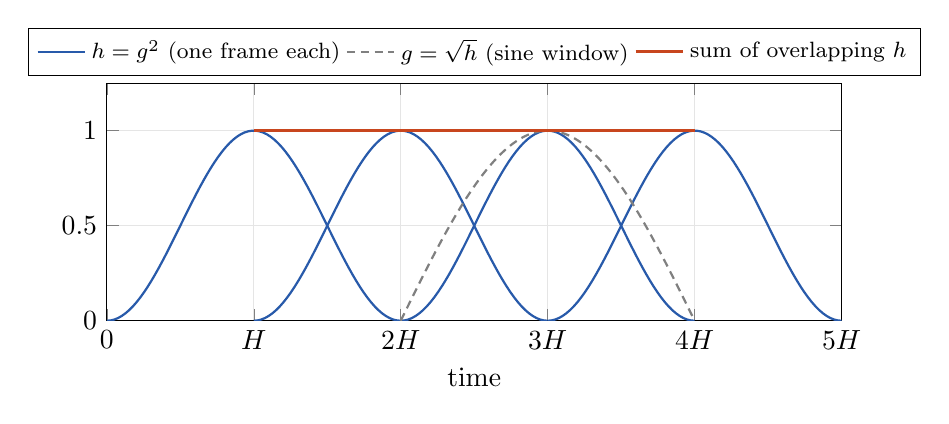
\begin{tikzpicture}
\begin{axis}[width=0.9\linewidth, height=4.6cm, xmin=0, xmax=2.5, ymin=0, ymax=1.25,
  xtick={0,0.5,...,2.5}, xticklabels={$0$,$H$,$2H$,$3H$,$4H$,$5H$}, ytick={0,0.5,1},
  xlabel={time}, grid=major, grid style={gray!20}, samples=80, legend columns=3,
  legend style={at={(0.5,1.03)}, anchor=south, font=\footnotesize}]
  \addplot[thick, dascol, domain=0:1] {sin(deg(pi*x))^2};
  \addlegendentry{$h=g^2$ (one frame each)}
  \addplot[thick, dascol, domain=0.5:1.5, forget plot] {sin(deg(pi*(x-0.5)))^2};
  \addplot[thick, dascol, domain=1:2, forget plot] {sin(deg(pi*(x-1)))^2};
  \addplot[thick, dascol, domain=1.5:2.5, forget plot] {sin(deg(pi*(x-1.5)))^2};
  \addplot[thick, gray, densely dashed, domain=1:2] {sin(deg(pi*(x-1)))};
  \addlegendentry{$g=\sqrt{h}$ (sine window)}
  \addplot[very thick, sdcol, domain=0.5:2] {1};
  \addlegendentry{sum of overlapping $h$}
\end{axis}
\end{tikzpicture}
\caption{50\%-overlapped periodic Hann windows sum to exactly one (Proposition~\ref{prop:cola}).
The time axis is in hops; each frame spans $N=2H$ samples.}
\label{fig:cola}
\end{figure}

\begin{figure}[ht]
\centering
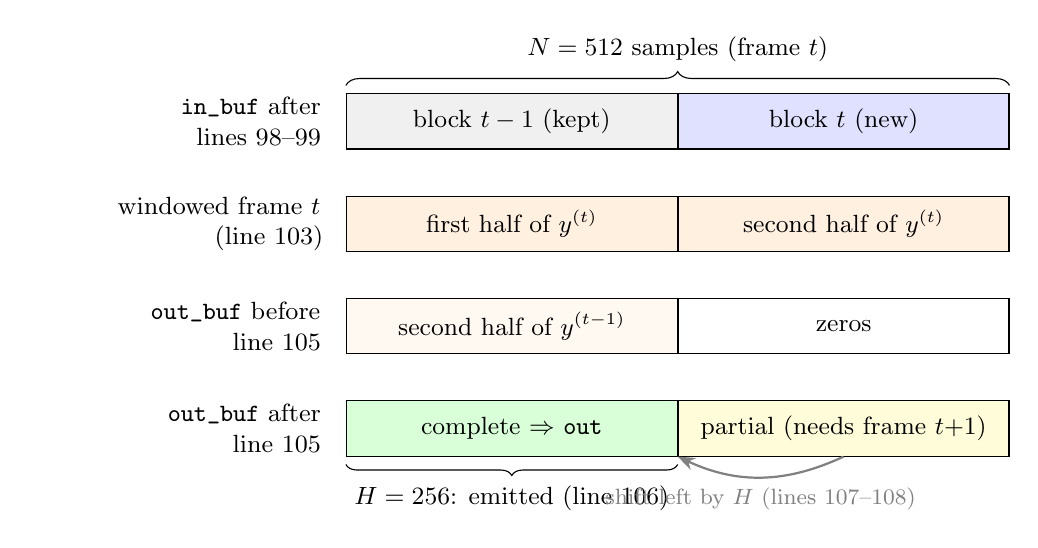
\begin{tikzpicture}[cell/.style={draw, minimum height=7mm, minimum width=42mm, font=\small, align=center},
                    lab/.style={font=\small, anchor=east, align=right, text width=36mm}]
  \node[lab] at (-0.2,0) {\code{in_buf} after\\lines 98--99};
  \node[cell, fill=gray!12, anchor=west] (a1) at (0,0) {block $t-1$ (kept)};
  \node[cell, fill=blue!12, anchor=west] (a2) at (a1.east) {block $t$ (new)};
  \node[lab] at (-0.2,-1.3) {windowed frame $t$\\(line 103)};
  \node[cell, fill=orange!12, anchor=west] (b1) at (0,-1.3) {first half of $y^{(t)}$};
  \node[cell, fill=orange!12, anchor=west] (b2) at (b1.east) {second half of $y^{(t)}$};
  \node[lab] at (-0.2,-2.6) {\code{out_buf} before\\line 105};
  \node[cell, fill=orange!5, anchor=west] (c1) at (0,-2.6) {second half of $y^{(t-1)}$};
  \node[cell, anchor=west] (c2) at (c1.east) {zeros};
  \node[lab] at (-0.2,-3.9) {\code{out_buf} after\\line 105};
  \node[cell, fill=green!15, anchor=west] (d1) at (0,-3.9) {complete $\Rightarrow$ \code{out}};
  \node[cell, fill=yellow!15, anchor=west] (d2) at (d1.east) {partial (needs frame $t{+}1$)};
  \draw[decorate, decoration={brace, amplitude=5pt}] ($(a1.north west)+(0,0.1)$) -- ($(a2.north east)+(0,0.1)$)
       node[midway, above=5pt, font=\small] {$N=512$ samples (frame $t$)};
  \draw[decorate, decoration={brace, amplitude=4pt, mirror}] ($(d1.south west)-(0,0.1)$) -- ($(d1.south east)-(0,0.1)$)
       node[midway, below=4pt, font=\small] {$H=256$: emitted (line 106)};
  \draw[arr, gray] (d2.south) to[bend left=25] node[below, font=\footnotesize] {shift left by $H$ (lines 107--108)} (d1.south east);
\end{tikzpicture}
\caption{Buffer bookkeeping in one call to \code{process}. Output block $t$ is input block $t-1$,
filtered, so the algorithm adds exactly $H$ samples of delay.}
\label{fig:buffers}
\end{figure}

\subsection{Circular convolution and how much it matters}

Multiplying DFT bins is \emph{circular} convolution. Each mic is convolved with the length-$N$
impulse response $\mathrm{h}_m=\code{irfft}(\overline{w_{\cdot,m}})$, and any part of that
response that extends past the frame edge wraps around to the other end. For DAS the responses
are fractional delays of at most 6 samples, so the wrap is negligible. The superdirective
responses are longer. Measured from \texttt{design\_weights} over all seven mics, $91\%$ of
their energy lies within $\pm32$ samples of $n=0$ and $99.8\%$ within $\pm128=\pm N/4$.
The synthesis half of the sine window tapers both frame edges to zero, which further
attenuates whatever wraps. So the residual time-aliasing is small but not zero. Eliminating it
completely would require constraining the filter length or zero-padding the FFT
($N_{\text{fft}}>N$), at some cost in latency and CPU.

\begin{remark}
\code{irfft} ignores the imaginary parts of the DC and Nyquist (24\,kHz) bins, because a real
signal cannot have them. The weights are real at DC (Section~\ref{sec:loading}). At 24\,kHz they
are not exactly real, but that bin is far above anything the MEMS mics or the ear contribute.
\end{remark}

\begin{rationale}[s for the STFT]
\begin{itemize}
\item \textbf{$\sqrt{\text{Hann}}$ on both sides.} The analysis taper limits spectral leakage
  between bins. The synthesis taper makes each processed frame fade in and out, so changes in
  the frame's content never produce edge discontinuities (clicks), and it suppresses circular
  wrap. COLA only constrains the \emph{product} $g_a g_s$, so the symmetric split $g_a=g_s=\sqrt h$
  gives both benefits.
\item \textbf{Periodic, not symmetric, Hann.} \code{np.hanning(N)} uses denominator $N-1$, and
  then $h[n]+h[n+H]\neq1$, which leaves a small ripple at the hop rate. The \code{N+1}/\code{[:-1]}
  trick on line~91 makes the identity exact.
\item \textbf{50\% overlap ($N=2H$).} This is the least overlap for which the sine-window pair
  satisfies COLA. It costs one FFT per channel per hop, the minimum possible.
\item \textbf{$H=256$ at 48\,kHz.} This gives an algorithmic latency of $H/f_s=5.33$\,ms (plus
  device buffering) and a bin spacing of $f_s/N=93.75$\,Hz. Halving $H$ would halve the latency
  but give only 2--3 bins below 300\,Hz, exactly where superdirectivity earns its keep. Doubling
  $H$ would give finer bins but 10.7\,ms of latency, which becomes noticeable when you can also
  hear the room directly.
\item \textbf{The \code{frames != BLOCK_SIZE} guard} (line~139) outputs silence for an odd-sized
  callback, because the overlap-add bookkeeping assumes a fixed hop.
\item \textbf{Implementation details.} Conjugating the weights once (line~92) moves that work out
  of the callback. \code{float32}/\code{complex64} halves memory traffic and matches the stream's
  dtype; float32's 24-bit mantissa already exceeds a 24-bit converter's resolution.
  \code{.copy()} on line~106 is required: \code{out_buf[:h]} is a view, and line~107 overwrites
  it in place.
\end{itemize}
\end{rationale}

% =============================================================================
\section{Gain staging, output and level metering}\label{sec:gain}
% =============================================================================

\demolines{135}{147}

\demolines{200}{201}

Because the beamformer is distortionless ($\vw\herm\vd=1$, Section~\ref{sec:das}), the target passes
through it at unity gain. All of the loudness therefore comes from one scalar,
\begin{equation}
  G=\code{OUTPUT_GAIN}\cdot2^{s}=8\cdot2^{1}=16,\qquad 20\log_{10}16=24.08\ \text{dB},
\end{equation}
where $s$ is \code{--gain-shift}, and each step of $s$ adds $20\log_{10}2=6.02$\,dB.
In IEEE-754 floating point, multiplying by $2^{s}$ changes only the exponent field, so it is
exact: the floating-point analogue of a left shift by $s$ bits. Since $8=2^3$ as well, $G$ is a
power of two and the scaling adds no rounding error at all.

\begin{rationale}[s for the output stage]
\begin{itemize}
\item \textbf{Why so much gain.} The RAW firmware (\code{micArray_vf_raw}) applies no digital
  gain, and MEMS mics at conversational distances sit far below full scale.
\item \textbf{Why clip} (line~146). Values outside $[-1,1]$ would be wrapped or otherwise mangled
  by the output path. A hard clip limits the damage to brief distortion during overloads. It
  does nothing at normal levels.
\item \textbf{Why mono to both ears} (line~147). A beamformer produces one signal. Feeding it to
  both ears centres the voice in the head; the array's spatial cues are not preserved.
\end{itemize}
\end{rationale}

\paragraph{Level metering (\code{--levels}).} Lines~157--158 print, for each channel, the
level in dB relative to full scale over a 100\,ms block:
$L=20\log_{10}\!\big(\sqrt{\tfrac1n\sum x^2}\big)$\,dBFS. A full-scale sine reads
$-3.01$\,dBFS, a silent channel reads about $-240$\,dBFS (from the $10^{-12}$ floor), and
tapping a mic makes its channel jump by tens of dB. This is how you verify the channel mapping
assumed on lines~20--27.

% =============================================================================
\appendix
\section{Parameters and their effects}\label{app:params}
% =============================================================================

\begin{center}\small
\begin{tabular}{@{}>{\raggedright}p{3.6cm}l>{\raggedright\arraybackslash}p{8.4cm}@{}}
\toprule
Constant (line) & Value & Meaning; effect of changing it\\
\midrule
\code{SAMPLE_RATE} (6) & 48000 & $f_s$. Sets bin spacing $f_s/N$ and latency $H/f_s$.\\
\code{IN_CHANNELS} (7) & 8 & 7 mics + spare, as delivered by the RAW firmware.\\
\code{OUT_CHANNELS} (8) & 2 & Headphones; both get the same mono beam.\\
\code{BLOCK_SIZE} (9) & 256 & Hop $H$; FFT is $2H$. Larger: finer bins, more latency.\\
\code{RING_MIC_ANGLES_DEG} (20) & see Fig.~\ref{fig:array} & Mic angles $\theta_m$. Must match the hardware, or the beam mis-steers.\\
\code{RING_RADIUS} (29) & 0.043 m & $r$. Sets all spacings, the aliasing limit and low-frequency directivity.\\
\code{LOOK_AZIMUTH_DEG} (31) & 0 & $\phi_0$. Steers the beam; any angle works because $\vd$ is computed, not tabulated.\\
\code{SPEED_OF_SOUND} (32) & 343 m/s & $c$ at about $20^\circ$C. A few-\% error slightly mis-scales $\tau_m$.\\
\code{DIAGONAL_LOADING} (33) & 0.05 & $\mu$. Higher: less hiss, wider beam (tends to DAS). Lower: narrower beam, more hiss.\\
\code{OUTPUT_GAIN} (34) & 8 & Fixed post-beam gain (18.1 dB).\\
\code{GAIN_SHIFT_BITS} (35) & 1 & Default \code{--gain-shift}; $+6.02$ dB per step.\\
\bottomrule
\end{tabular}
\end{center}

\section{Symbols}
\begin{center}\small
\begin{tabular}{@{}ll@{\qquad}ll@{}}
\toprule
$M$ & number of mics (7) & $\vp_m$ & position of mic $m$\\
$f_s$ & sample rate & $\vu$ & unit vector toward source\\
$H,\ N$ & hop (256), FFT length (512) & $\tau_m$ & arrival advance at mic $m$\\
$k,\ f_k$ & bin index, $k f_s/N$ & $\kappa$ & wavenumber $2\pi f/c$\\
$\phi,\ \phi_0$ & azimuth, look azimuth & $\vd(f,\phi)$ & steering vector\\
$\vw(f)$ & beamformer weights & $\G,\ \Gmu$ & diffuse coherence, loaded\\
$\mu$ & diagonal loading & $B(f,\phi)$ & beam pattern $\vw\herm\vd$\\
$\WNG$ & white-noise gain $1/\|\vw\|^2$ & $\DI$ & diffuse array gain\\
$g,\ h$ & sine window, periodic Hann & $G$ & output gain $8\cdot2^s$\\
\bottomrule
\end{tabular}
\end{center}

\end{document}
